\def\year{2021}\relax
%File: formatting-instruction.tex
\documentclass[letterpaper]{article} % DO NOT CHANGE THIS
\usepackage{aaai20}  % DO NOT CHANGE THIS
\usepackage{times}  % DO NOT CHANGE THIS
\usepackage{helvet} % DO NOT CHANGE THIS
\usepackage{courier}  % DO NOT CHANGE THIS
\usepackage[hyphens]{url}  % DO NOT CHANGE THIS
\usepackage{graphicx} % DO NOT CHANGE THIS
\usepackage{makecell}
\usepackage{amsmath}
\usepackage{breqn}
\usepackage{lipsum}
\usepackage{subcaption}
\usepackage{amssymb}
\usepackage{courier}
\usepackage[ruled,vlined]{algorithm2e}
\usepackage{multirow}
\urlstyle{rm} % DO NOT CHANGE THIS
\def\UrlFont{\rm}  % DO NOT CHANGE THIS
\usepackage{graphicx}  % DO NOT CHANGE THIS
\frenchspacing  % DO NOT CHANGE THIS
\setlength{\pdfpagewidth}{8.5in}  % DO NOT CHANGE THIS
\setlength{\pdfpageheight}{11in}  % DO NOT CHANGE THIS

%\nocopyright
%PDF Info Is REQUIRED.
% For /Author, add all authors within the parentheses, separated by commas. No accents or commands.
% For /Title, add Title in Mixed Case. No accents or commands. Retain the parentheses.
 \pdfinfo{
/Title (Data driven robust optimization for planning and replanning the Lot-sizing and scheduling problems: Machine learning approach)
/Author (Mohammad Rohaninejad, Mikoláš Janota, Zdeněk Hanzálek)
} 
\setcounter{secnumdepth}{0} %May be changed to 1 or 2 if section numbers are desired.

% The file aaai20.sty is the style file for AAAI Press 
% proceedings, working notes, and technical reports.
%
\setlength\titlebox{2.5in} % If your paper contains an overfull \vbox too high warning at the beginning of the document, use this
% command to correct it. You may not alter the value below 2.5 in
\title{Data driven robust optimization for planning and replanning the Lot-sizing and scheduling problems: Machine learning approach}
%Your title must be in mixed case, not sentence case. 
% That means all verbs (including short verbs like be, is, using,and go), 
% nouns, adverbs, adjectives should be capitalized, including both words in hyphenated terms, while
% articles, conjunctions, and prepositions are lower case unless they
% directly follow a colon or long dash
\author{Mohammad Rohaninejad\textsuperscript{\rm 1}, Mikoláš Janota \textsuperscript{\rm 2}\textsuperscript{\rm ,1}, Zdeněk Hanzálek\textsuperscript{\rm 1}
\\
\textsuperscript{\rm 1}Czech Institute of Informatics, Robotics, and Cybernetics, Czech Technical University in Prague\\
\textsuperscript{\rm 2}INESC-ID/IST, Universidade de LisboaLisbonPortugal\\
}
 \begin{document}

\maketitle

\begin{abstract}
This paper develops a new data-driven robust approach based on machine learning for the dynamic lot-sizing and scheduling problem. The system learns in a manufacturing environment by using machine learning to tackle the challenge of demand and processing time uncertainty. The SMT based formulation of the problem is developed for the job shop system considering the sequence-dependent setup time. Then a robust solution procedure has been proposed with combination of the repression neural network and a K-mean based heuristic. This procedure is based on determining the profitable value of safety stock and safety slack levels as a strategy for creating robustness.We also developed a Monte Carlo simulation to assess the performance of proposed robust approach comparing the worst-case scenario, average-scenario and also deterministic rolling planning approaches. Computational results show that proposed approach is effective and considerably better than other approaches to producing less nervous and feasible solutions. 
\end{abstract}



\section{Introduction}

Integrated lot-sizing and scheduling (ILSP) is one of the most important and frequently-used problems in production planning which are considered among medium-term or long-term planning (Rohaninejad et al. 2015). In ILSP two types of decision variables including the master planning variables (how much of jobs should be produce in which periods) and variables related to the detailed schedule (sequence of jobs within the periods) are usually determined during a finite planning horizon. The capacitated lot-sizing and scheduling problem (CLSP) is NP-hard (Bitran and Yanasse 1982). In addition finding the feasible solution for CLSP is as well NP-hard (Maes et al. 1991). This complexity will intensify in a dynamic environment so that meeting the client’s delivery time (without shortage) is often very difficult in dynamic CLSP. In dynamic environments the initial plans are immediately affected by unpredictable noise such as demand or processing time fluctuations, machines breakdown, due date changes, order cancellation, etc. These disruptions are generally replanning or rescheduling triggers and usually cause to update of decision variables via a rolling  planning (RP) manner. Predictive, completely reactive, and mixed predictive-reactive are the three common strategies to deal the production planning with uncertainty. In the predictive or predictive-reactive strategies all or some decisions regarding control variables are made in advance and remained control variables are revised in response to real-time events. These strategies require a minimum level of prediction and information regarding distribution function. However, the majority of real-life applications are indeed dynamic due to uncontrollable and hard-to-predict events (Baykasoğlu and Ozsoydan 2018). Nevertheless, the completely reactive rescheduling is widely applicable while all control variables are revised in response of real-time disruptions. Preserving the feasibility in the completely reactive rescheduling is very hard because of the high sensitivity of schedule provided in advance (original plans) to the change of data. Therefore, increasing the resiliency of the original plan to absorb the effect of disruptions is a natural reaction to that can be achieved by the robust optimization approach. Robust optimization is an effective approach to producing less nervous solutions with less need for revision in different situations.  Data driven robust production planning is a new paradigm that is formed as a result of explosion in the availability of data during last decade. This approach uses the  historical data while are available from a discrete event simulation or real production for interpretation of the probability function and uncertainty behavior.
This paper proposes a completely reactive strategy for scheduling and rescheduling of the dynamic CLSP in job shop under the demand and processing time uncertainty. The rescheduling algorithm is implemented in a periodic pattern in the first of each period considering the new realized data. This algorithm is based on a new data-driven robust model under satisfiability modulo theory (SMT) while some parameters of the model are updated using  machine learning (ML). 

\section{Literature review}
The scheduling decisions are not integrated into the classical lot-sizing problems and the usual approach, therefore, is to solve lot-sizing problems first and then solve scheduling for each period separately afterward (Drexl and Kimms 1997). Discrete lot-sizing and scheduling (DLSP), continuous setup lot-sizing problem (CLSP), proportional lot-sizing and scheduling problem (PLSP) and general lot-sizing and scheduling problem (GLSP) are some attempts to integrate them. For a detailed review of these models see (Drexl and Kimms 1997).\\
Thereafter, several studies have been done for considering different type of uncertainty in the ILSP such as demand uncertainty (Hu and Hu 2016), lead time uncertainty (Rahdar et al. 2018), processing and setup time uncertainty (Ramezanian and Saidi-Mehrabad 2013), due dates uncertainty (Petrovic et al. 2005), random machine breakdown (Dolgui et al. 2010), random products rejection (Schemeleva et al. 2012), random workforce efficiency (Li and Hu 2017) etc. Although most of them are based on pre-active stochastic or fuzzy scheduling to overcome uncertainty in the original scheduling without any real-time response. Creating robust scheduling  is not possible by completely pre-active scheduling in many of real-life applications. Therefore rescheduling or online scheduling problems have attracted a lot of attention during the last decade. The rescheduling problem has been studied widely in purely scheduling problems in shop floor (for detailed review see Gupta et al. (2016)) but there are few studies of rescheduling in the ILSP. Haase and Kimms (2000) are presented an efficient rescheduling approach for single machine ILSP with sequence dependent setup time and demand uncertainty. They have developed a Branch-and-Bound method to solve the remaining sub-problem and reveal the optimal solution. Curcio et al. (2018) have proposed an adjustable robust optimization to adjust the size and sequence of lot variables in every period. They have used the Monte Carlo simulation to evaluate the proposed method. Rolling horizon is an other approach to deal with uncertainty in the ILSP (Vargas and Metters 2011; Saif rt al. 2019; Tiacci and Saetta 2012). In each iteration of Rolling horizon usually the scheduling decisions related to the closer period are obtained in detail and on later periods are only represented in the master level. Then the master scheduling of later periods will be detailed after observation of uncertain data in the next iterations.
In term of robust optimization in ILSP, there are  several studies (Curcio et al. 2018; Alem et al. 2018). Data-driven robust optimization is widely raised in recent years. This approach is flexible, applicable and computationally tractable in the different research fields specially in scheduling problem (Zhang et al. 2018a;Zhang et al. 2018b;He et al. 2019). Jiang and Guan (2016) have developed a data-driven robust optimization to provide robust solutions for the chance constrained stochastic program in classical capacitated lot-sizing problem.
computing the surrogate models is one of the most applications of ML in data-driven optimization (For more information see Jin et al. (2018)). ML is used in several manners in the scheduling problems such as selecting the parameters of heuristic (Mönch et al. 2006), resources dispatching (Chen and Yen 2011), selection of the best solving algorithm (de León et al. 2017), predict consequences of scheduling decisions (Berral et al. 2010), learning constraint's parameters (Picard-Cantin et al. 2016), etc. Finding the best dispatching rule application of the ML techniques in the dynamic scheduling and rescheduling problems (Metan and Sabuncuoglu 2005; Mouelhi-Chibani and Pierreval 2010; Shiue 2009). Based on our knowledge there is not any benchmark study that has been investigated the data-driven robust optimization and also ML for the rescheduling in ILSP and this paper is the first effort to extend data-driven robust scheduling for ILSP using ML.

\section{Problem description}
This paper investigates ILSP in the job shop problems with $M$ capacitated machines and sequence dependent setup time. The planning horizon contains finite periods while the value of parameters in each period may differ than other periods. Furthermore, the following assumptions are applied:

\begin{quote}
\begin{itemize}
\item Machines are available all the time.
\item Machines can at the most process one job at a time.
\item An operation can be done only one time in a period.
\item The consumption coefficient between different levels of jobs is set to 1.
\item Due dates of all orders are deterministic within the end of each periods.
\item There are no interruptions in operations processing.
\item Product delivery cannot be split and shortage in not allowed.
\end{itemize}
\end{quote}

\section{SMT formulation (deterministic model)}
In this section, the SMT formulation of ILSP is presented for the job shop problem. In this model the operation $o$ of job $j$ is noted by \textit{$O_{jo}$}. The other detailed information of the model is as follows.\\\\
\iffalse
\textbf{Indices}\\
\parbox{30pt}{\textit{j,j$'$,k}} 
\parbox{208pt}{Index of jobs (\textit{j,j$'$,k=1,..,J})}\\
\parbox{30pt}{\textit{o,o$'$,l}}
\parbox{208pt}{Index of operations}\\
\parbox{30pt}{\ $h_{j}$}
\parbox{208pt}{Last operation of job  (\textit{j})}\\
\parbox{30pt}{\textit{m}}
\parbox{208pt}{Index of machines (\textit{m=1,..,M})}\\
\parbox{30pt}{\textit{t}}
\parbox{208pt}{Index of periods  (\textit{t=1,..,T})}\\
\\
\fi
\textbf{Parameters}\\
\parbox{30pt}{\textit{$D_{jt}$}} 
\parbox[t]{207pt}{Demand for job \textit{j} during period \textit{t}}\\
\parbox{30pt}{\textit{$p_{jo}$}} 
\parbox[t]{207pt}{Processing time needed to produce one unit of $O_{jo}$}\\
\parbox{30pt}{\textit{$C_{mt}$}} 
\parbox[t]{207pt}{Capacity of machine \textit{m} during period \textit{t}}\\
\parbox{30pt}{\textit{$\delta_{joj'o'}$}} 
\parbox[t]{207pt}{Setup time of $O_{jo}$ if processed immediately after $O_{j'o'}$ on a same machine}\\
\parbox{30pt}{\textit{$a_{jo}$}} 
\parbox[t]{207pt}{Machine, which is supposed to process $O_{jo}$}\\
\parbox{30pt}{\textit{L}} 
\parbox[t]{207pt}{Length of each period}\\
\\
\textbf{Variables}\\
\parbox{30pt}{\textit{$x_{jot}$}} 
\parbox[t]{207pt}{Quantity of $O_{jo}$ that is produced in period \textit{t}}\\
\parbox{30pt}{\textit{$s_{jot}$}} 
\parbox[t]{207pt}{Start time regarding $O_{jo}$ in period \textit{t}}\\
\parbox{30pt}{\textit{$I_{jot}$}} 
\parbox[t]{207pt}{Amount of inventory of $O_{jo}$ at the end of period \textit{t}}\\

With the notations introduced above, the problem can be formulated in the SMT format  as follows:
\begin{equation}
I_{j h_j t-1}+x_{j h_j t} - I_{j h_j t} = D_{jt} \quad\quad  \forall t, \forall j
\end{equation}
\begin{equation}
I_{j o t-1}+x_{j o t} - I_{j o t} = x_{j o+1 t}
\end{equation}
\begin{equation}
(I_{j o t-1}+x_{j o+1 t} \geq 0) \vee  (s_{j o+1 t} \geq s_{jot}+x_{jot}p_{jo})
\end{equation}
$$\forall t, \forall j,o=1,...,h_{j}-1$$
\begin{equation}
\sum_{j=1}^{J} \sum_{o=1|a_{jo}=m}^{h_{j}} x_{j o t} p_{jo} \leq C_{mt} \quad\quad  \forall t, \forall m
\end{equation}
\iffalse
\begin{multline}
\Big( s_{jot} \geq s_{j'o't} + x_{j'o't} p_{j'o'}+ \delta_{joj'o'} 
\\
\vee s_{j'o't}\geq s_{jot} + x_{jot} p_{jo} + \delta_{j'o'jo} \Big) \vee
\\
\bigvee\limits_{\substack{kl \neq jo \neq j'o' \\ a_{kl} = a_{jo}= a_{j'o'}}} \Big( \big( s_{klt} \geq s_{jot} + x_{jot} p_{jo}+ \delta_{kljo} \wedge s_{j'o't}\geq
\\
s_{klt} + x_{klt} p_{kl} + \delta_{j'o'kl} \big) \vee \big( s_{jot} \geq s_{klt} + x_{klt} p_{kl}+ \delta_{jokl} 
\\
\wedge s_{klt}\geq s_{j'o't} + x_{j'o't} p_{j'o'} + \delta_{klj'o'} \big) \Big)                       
\end{multline}
\fi
\begin{multline}
\Big( (s_{jot} \geq s_{j'o't} + x_{j'o't} p_{j'o'}+ \delta_{joj'o'}) \vee
\\
(s_{j'o't}\geq s_{jot} + x_{jot} p_{jo} + \delta_{j'o'jo}) \Big)\vee\chi_{joj'o'}^{(t)}
\end{multline}
$$\forall t, \forall O_{jo}, \forall O_{j'o'},
O_{jo}\neq O_{j'o'},a_{jo}=a_{j'o'}$$
\begin{equation}
(s_{jot} \geq (t-1)L) \vee  (s_{jot}+x_{jot}p_{jo} \leq tL) \quad  \forall t, \forall O_{jo}
\end{equation}
%\begin{equation}
%Min \left(\sum_{t=1}^{T} \sum_{j=1}^{J} \sum_{o=1}^{h_{j}} zs_{jot}+zp_{jot}+zh_{jot} \right)
%\end{equation}

The inventory balance regarding the last operation of each job, between periods, is ensured in Constraint (1); Constraint (2) shows the balance for other operations. Constraints (3) guarantees the $O_{jo}$ should proceed before the $O_{jo+1}$ in period $t$ if there is no minimum required inventory of this operation at the end of period $t-1$. The capacity restriction of each machine is respected in Constraint (4). Constraints (5) determines the sequence of $O_{jo}$ and $O_{j'o'}$ with same machine in period $t$ considering the sequence dependent setup time. In this constraint $\chi_{joj'o'}^{(t)}$ is an alternative variable for simplifying the model. This variable is equal to 1 if there is at least one operation between $O_{jo}$ and $O_{j'o'}$ in period $t$; otherwise is equal to 0 (The equivalent SMT formulation of $\chi_{joj'o'}^{(t)}$ is presented in the appendix). Constraints (6) specify the restrictions of start time and finish time of each operation within period $t$.

\section{Data Driven Robust approach}
There are some drawbacks to rescheduling or reactive dynamic scheduling. Creating the feasibility conditions in rescheduling is the main obstacle to provide a new schedule. In schedule repair or complete rescheduling, the main question is if the available resources are enough for feasible rescheduling or not? This paper presents a new approach to determine the safety value of stock and slack (2-SS) as a strategy to satisfy the feasibility of solutions after changes of demand or processing time. Although this strategy may lead to extremely conservative and costly solutions. For example, in the ILSP, the inventory holding cost will be extremely increased by considering the high level of safety stock. On the other side, the high-risk solutions (risk of infeasibility) and subsequently cost of shortage or unmet demands will be increased when we consider the low level of safety stock. Indeed, the decision-maker should strike a balance between the risk of infeasibility and another system costs. For this reason, our strategy combined with a regression neural network algorithm and a K-Mean based heuristic for finding a reliable and cost-efficient value of 2-SS through the adaption of existing data and historical data. 

\subsection{2-SS approach}
Figure 1 shows how more lot-size and idle time as  safety stock and safety slack can made the initial plan robust against the possible increase in demand and processing time. In this figure, each task illustrated by $O_{jo}$ and as well the size of lot inside parentheses. In figure 1.a the deterministic plan with optimal value of completion time  is displayed without considering the demand and processing time uncertainty. In figures 1.b and 1.c the resilience of the plan (1.a) has been strengthened by increasing the amount of lot as safety stock and amount of idle time as safety slack with completion time equal to 37.
\begin{figure}[t]
\begin{subfigure}{.46\textwidth}
  \centering
  \captionsetup{justification=centering}
  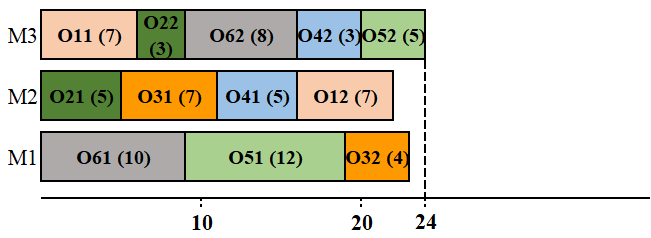
\includegraphics[width=0.9\columnwidth]{figure/fig2-1.png} %
  \caption{Deterministic plan according to observed data}
  \label{fig:fig1-1}
\end{subfigure}
\begin{subfigure}{.46\textwidth}
  \centering
  \captionsetup{justification=centering}
  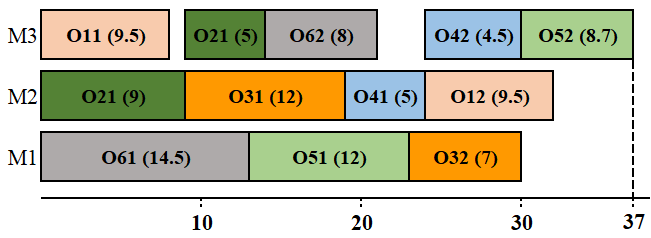
\includegraphics[width=0.9\columnwidth]{figure/fig2-2.png} %
  \caption{Reliable plan by increasing amount of lot as safety stock}
  \label{fig:fig1-2}
\end{subfigure}
\begin{subfigure}{.46\textwidth}
  \centering
  \captionsetup{justification=centering}
  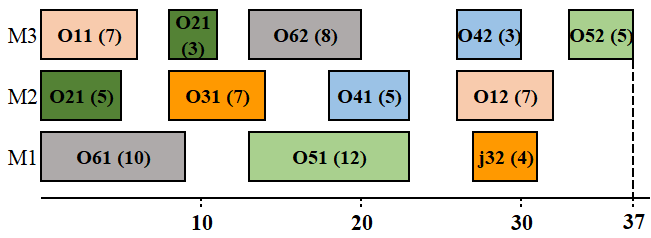
\includegraphics[width=0.9\columnwidth]{figure/fig3-2.png} %
  \caption{Reliable plan by increasing idle time as safety slack}
  \label{fig:fig1-3}
\end{subfigure}
\caption{2-SS approach for robust planning against the possible increase in demand and processing time}
\label{fig2}
\end{figure}

\subsection{Neural network}
The uncertainty behavior is a function of several factors in the production planning environment. These factors can be dependent or independent and can have synergies in influencing the distribution function. For example, the amount of demand can be a function of different components such as periods of time, seasonal changes, product life cycle, advertising and marketing plans, the performance of competitors, order rate and returned product rate in previous periods, etc. Similarly, the processing time of work can be affected by factors such as assigned machine or operator to the work, the volume of loaded works, the time spent without maintenance operation, physical and chemical and environmental conditions, etc. 
Learning is one mechanism for identification and discovery the complex interaction between these factors. This paper is developed a regression neural network (NN) for distribution interpretation. we have considered the total rate of realized orders in the last periods, current period and also the period number as three effective factors on the demand distribution. The higher value of the order rate in previous and current periods can provide a higher value of demand in the next periods and vice versa. There is more correlation between the random demands in current period with the observed order rate in the same period than previous periods. For the third factor, the different demand rate is considered in different periods. The rate of machine idle time is also considered as an effective factor on the processing time. The more value of idle time as a time for doing machine services can provide less processing time. The NN that used here is composed of two separate networks. One is related to safety stock and another is related to safety slack prediction. Each of them are trained separately based on their specific input and output value. The meanings of the input and output value for both networks are shown in Table 1. The structure of the two networks is the same including one input layer, two hidden layers, and one output layer.

\begin{table}[t]
\scriptsize
\caption{The input and output layer value for proposed neural networks}\smallskip
\centering
%\resizebox{.95\columnwidth}{!}{
\smallskip\begin{tabular}{ccc}
\hline
Network  & Input  & Output  \\
\hline
\makecell{ Network 1 \\ (safety stock\\ prediction)}
 & \makecell{ 1)	Total realized orders \\in previous periods \\
2)	Total realized order \\ in current period\\ 
3)	Current period number }
 & \makecell{ 1)	Global optimum \\inventory level \\ considering all realized \\ orders in the sample } \\
 \hline
\makecell{ Network 2 \\ (safety slack \\ prediction)}
 & \makecell{ 1)Total machines idle \\ time in the last period }
 & \makecell{ $max\left\{0,\tilde{p}_{jo}-p_{jo}\right\}$} \\
 \hline
\end{tabular}
\label{table1}
\end{table}

Based on information represented in table 1 there are $2J+1$ nodes in the input layer of the neural network 1. There are $\sum_{j=1}^{J} h_{j}T$ nodes in the output layer of network 1 that correspond to global optimum inventory level ($I_{jot}^{*}$). We have to solve an optimization model with aim of minimization of system cost for each sample of training set considering the final observed demand. The obtained optimum values for inventories is used as value of nodes correspond to the output layer. Forasmuch as the proposed NN will be executed during the RP approach the size of the output layer will be changed and is equal to $\sum_{j=1}^{J} h_{j}(T-t+1)$ in iteration $t$ (current period = $t$). 
There are $M$ nodes in the input layer of the network 2.There are $\sum_{j=1}^{J} h_{j}$ nodes in the output layer of network 2 that correspond to $max\left\{0,\tilde{p}_{jo}-p_{jo}\right\}$ in each sample while $p_{jo}$ and $\tilde{p}_{jo}$ are the nominal and realized value of processing time for $O_{jo}$ respectively. In iteration $t$ of RP, there are two sub-networks for network 2 which one is responsible for the prediction of safety slack in period $t$ and another for period $t+1$. The periods greater than $t+1$ will be solved with nominal values of processing time. It should be noted that there is not any executed schedule for period $t$ in the iteration $t$ of proposed RP approach. Therefore, we have to use an approximation schema to estimate the machine’s idle time in period $t$ according to (7).
\begin{equation}
\sum_{j=1}^{J} \sum_{o=1|a_{jo}=m}^{h_{j}} \overline{x}_{jot}+S_{jot}^{+(t-1)}-S_{jot-1}^{+(t-1)}
\end{equation}
\parbox{30pt}{$S_{jot}^{+(t-1)}$} 
\parbox[t]{208pt}{The safety stock value that obtained by NN in iteration ($t-1$) of RP}\\
\parbox{30pt}{$\overline{x}_{jot}$} 
\parbox[t]{208pt}{Remained work (demand) related to operation $o$ of job $j$ that should be delivered in the end of period $t$}\\
According to $S_{jot}^{+(t-1)}$ and $S_{jot-1}^{+(t-1)}$ in relation (7) can be found that NN correspond to network 1 should be run before NN correspond to network 2.

\subsection{Model reformulation (robust model)}
For providing the robust formulation we have to reformulate the model presented previously. In the new model the constraint (8) is added to the model and the relation and constraints (3) to (6) are replaced with (9) to (12) respectively.

\begin{equation}
I_{jot}\geq S_{jot}^{+} - ps_{jot} \quad\quad  \forall t, \forall O_{jo}
\end{equation}
\begin{equation}
(I_{j o t-1}+x_{j o+1 t} \geq 0) \vee  (s_{j o+1 t} \geq s_{jot}+\xi_{jot})
\end{equation}
$$\forall t, \forall j,o=1,...,h_{j}-1$$
\begin{equation}
\sum_{j=1}^{J} \sum_{o=1|a_{jo}=m}^{h_{j}} \xi_{j o t} \leq C_{mt}  \quad\quad  \forall t, \forall m
\end{equation}
\iffalse
\begin{multline}
\Big( s_{jot} \geq s_{j'o't} + \xi_{j'o't}+ \delta_{joj'o'} 
\\
\vee s_{j'o't}\geq s_{jot} + \xi_{jot}+ \delta_{j'o'jo} \Big) \vee
\\
\lnot \bigg( \bigwedge\limits_{\substack{kl \neq jo \neq j'o' \\ a_{kl} = a_{jo} = a_{j'o'}}} \Big( \big( s_{klt} \geq s_{jot} + \xi_{jot}+ \delta_{kljo} \vee s_{j'o't}\geq
\\
s_{klt} + \xi_{klt} + \delta_{j'o'kl} \big) \vee \big( s_{jot} \geq s_{klt} +\xi_{klt}+ \delta_{jokl} 
\\
\vee s_{klt}\geq s_{j'o't} + \xi_{j'o't} + \delta_{klj'o'} \big) \Big) \bigg)                       
\end{multline}
\fi
\begin{multline}
\Big( s_{jot} \geq s_{j'o't} + \xi_{j'o't}+ \delta_{joj'o'} 
\\
\vee s_{j'o't}\geq s_{jot} + \xi_{jot}+ \delta_{j'o'jo} \Big)\vee\chi_{joj'o'}^{(t)}  
\end{multline}
$$\forall t, \forall O_{jo}, \forall O_{j'o'},
O_{jo}\neq O_{j'o'},a_{jo}=a_{j'o'}$$
\begin{equation}
(s_{jot} \geq (t-1)L) \vee  (s_{jot}+\xi_{jot} \leq tL) \quad  \forall t, \forall O_{jo}
\end{equation}
where : $\xi_{jot}=x_{jot}(p_{jo}+L_{jot}^{+}+pl_{jot})$
\\
$S_{jot}^{+}$ and $L_{jot}^{+}$ are the safety stock and safety slack value respectively. $ps_{jot}$ and $pl_{jot}$ are positive variable to obviate the infeasible situation that may be occurred by the value of $S_{jot}^{+}$ and $L_{jot}^{+}$ respectively.  

\subsection{Controlling the variation amplitude}
It can be found experimentally that using the NN is more reasonable if the variation amplitude of safety stock or safety slack is more restricted. The efficiency of NN degrades by increasing the variation amplitude in terms of the ability to maintain the feasibility of the problem. Figure 2 shows how a significant part of the possible scenarios can become infeasible when the realized values of a demand needs greater safety slack than estimated value (dashed line). The output values of the NN are largely dependent on the size of the training set. In the larger set, the output will be closer to the nominal value of random parameter and in the smaller set, deviation to one side is more likely. To address this challenge, we have combined NN with a heuristic based on K-mean clustering. The computational results confirm the improvement of NN performance in terms of feasibility. Algorithms 1 to 3 illustrate the pseudocodes of three consecutive part of proposed K-Mean based heuristic to cover the variation amplitude of safety stock. In this algorithm the $\pi$ and $\varphi$ are predefined value between 0 and 1 and also the value of $\vartheta_{jot}$ is calculated during the procedure as follow:
\\
$\vartheta_{jot}=\frac{\alpha-\beta}{\beta}$
\\
Where $\beta=\left(\frac{|\mathbb{M}_{jot}|}{ST} \right)$ and $Pr\left\{S_{jot}^{+}<\tilde{I}_{jot}\right\}\leq\alpha$\\
In the above relations, the $ST$ is the size of the training data set, $\tilde{I}_{jot}$ the true value that is required for safety stock after the realization of random data and also the $\alpha$ is the reliability coefficient that we are interested in the probability that the $\left(S_{jot}^{+}<\tilde{I}_{jot}\right)$ is violated be less than $\alpha$. 
\begin{figure}[t]
\centering
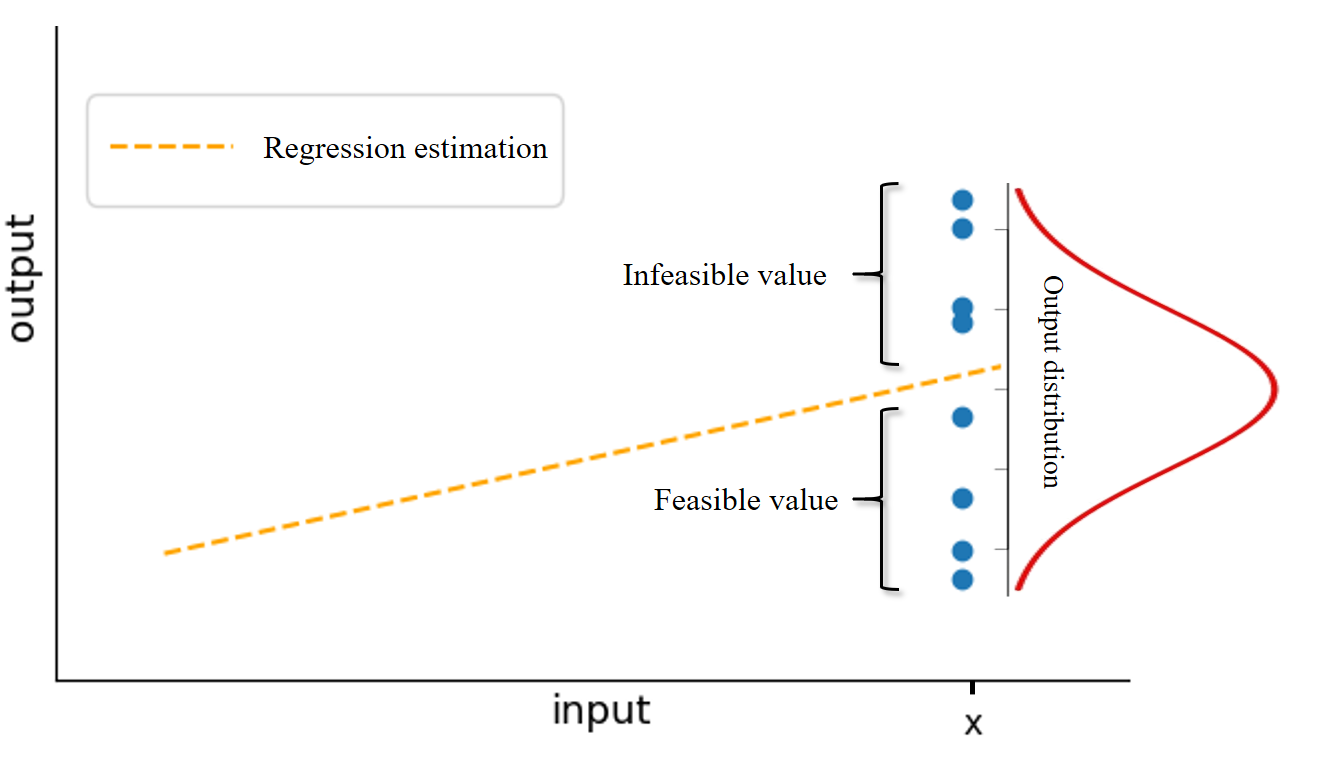
\includegraphics[width=0.9\columnwidth]{figure/fig4.png} % 
\caption{Feasible and infeasible scenarios based on regression estimation }
\label{fig3}
\end{figure}
\begin{algorithm}[t]
\SetAlgoLined
\KwResult{selection the potential data}
 update initial data including $t$, $x^{(t)}$ and $S_{jot}^{+}|\forall O_{j,o}$\;
 clustering training data by K-mean algorithm\;
 predict cluster of $x^{(t)}$ (cluster $k$)\;
 \For{each (j,o)}{
  $\mathbb{E}_{jot}\leftarrow\emptyset$ and $\mathbb{M}_{jot}\leftarrow\emptyset$\;
  \For{every data m in the $k^{th}$ cluster}{
  \If{$I_{jot}^{*(m)}-S_{jot}^{+(m)}>0$}{
   $\mathbb{E}_{jot}\leftarrow I_{jot}^{*(m)}-S_{jot}^{+(m)}$ and $\mathbb{M}_{jot}\leftarrow m$\;
   }
  }
 }
 \caption{K-mean based heuristic (part 1)}
\end{algorithm}
\begin{algorithm}[t]
\SetAlgoLined
\KwResult{set ($\mathbb{L}$) of operations $O_{j,o}$ to modify $S_{jot}^{+}$}
 $\mathbb{L}\leftarrow\emptyset$\;
 \While{$\exists \; (\mathbb{M}_{jot}\neq \emptyset)$}{
 Find ($j,o$) with maximum length of $\mathbb{M}_{jot}$\;
 \uIf{$\left(\frac{|\mathbb{M}_{jot}|}{\sum_{kl} |\mathbb{M}_{klt}|} \right)\geq \pi$}{
  $\mathbb{L},\mathbb{M}_{jot},\tau$=\texttt{final\_operations}($\mathbb{L},\tau,(j,o)$)\;}
\uElseIf{$\tau < \varphi$}{
   $\mathbb{L},\mathbb{M}_{jot},\tau$=\texttt{final\_operations}($\mathbb{L},\tau,(j,o)$)\;}
  \uElse{
   break \;
  }
  }

 \caption{K-mean based heuristic (part 2)}
\end{algorithm}
\begin{algorithm}[t]
\SetAlgoLined
\KwResult{modified safety stock value ($S_{jot}^{+}$)}
 \For{$\forall \; (j,o)\in \mathbb{L}$}{
\For{$\forall \; f\in \mathbb{E}_{jot}$}{
score($f$)=$\left(\frac{\sum_{f'\in\mathbb{E}_{jot}} 1 \left\{ f>f'\right\}}{|\mathbb{E}_{jot}|} \right)$ \;
}
find $f$ while is smallest member of $\mathbb{E}_{jot}$ and score($f$)$\geq\vartheta_{jot}$ then\;
$S_{jot}^{+}=S_{jot}^{+}+f$
  }

 \caption{K-mean based heuristic (part 3)}
\end{algorithm}
In the algorithm 1 the $t$, $x^{(t)}$ and $S_{jot}^{+}$ are current period number, The latest data realized until period $t$ and safety stock value obtained by NN respectively. In the \texttt{final\_operations} function of the algorithm 2, the values of $\mathbb{L}$, $\tau$ and $\mathbb{M}_{jot}$ are updated according to below relations while $\mathbb{L}$, $\tau$ and ($j,o$) are input parameters of function.\\
$\tau=\tau+\left(\frac{|\mathbb{M}_{jot}|}{\sum_{kl} |\mathbb{M}_{klt}|} \right)-\sum_{(j'o')\in \mathbb{L}} \left(\frac{|\mathbb{M}_{jot} \cap \mathbb{M}_{j'o't}|}{\sum_{kl} |\mathbb{M}_{klt}|} \right)+...+(-1)^n \sum_{(j'o',...,j^{n}o^{n})\in \mathbb{L}} \left(\frac{|\mathbb{M}_{jot} \cap \mathbb{M}_{j'o't}\cap ... \cap \mathbb{M}_{j^{n}o^{n}t}|}{\sum_{kl} |\mathbb{M}_{klt}|} \right)$\\
$\mathbb{L} \leftarrow (j,o)$\\
$\mathbb{M}_{jot} \leftarrow \emptyset$\\

A similar K-mean based heuristic is developed to encounter the variation amplitude of processing time.

\section{Computational results}
\subsection{Monte Carlo simulation}
A Monte Carlo simulation is developed to evaluate and compare the performance of proposed approach. During the simulation the proposed algorithm is implemented sequentially with realization of different random demands and processing time. The performance of different approaches is evaluated through the model robustness index (MRI\%) by determining what percentage of results are infeasible.


\subsection{Random data setting}
Algorithm 4 shows the pseudocode of random demand generation during the planning horizon. 
\begin{algorithm}[t]
\SetAlgoLined
\KwResult{updated value of realized demands}
\For{$j=1$ \hspace{.1cm} to \hspace{.1cm} $J$}{
\For{$t=\rho$ \hspace{.1cm} to \hspace{.1cm} $T$}{
$d_{j}=\left(\frac{d_{j}mc_{t}}{(t-\rho+1)} \right)$\;
\uIf {$t=\rho$} {
$d_{j}=d_{j}+\left(\frac{\tilde{D}_{jt}}{\left(\sum_{t'=1}^{\rho} \frac{d_{j}mc_{t}}{(t'+1)}\right)}-1 \right)0.5d_{j}$\;
}
\uElseIf {$t>\rho$} {
$d_{j}=d_{j}+\frac{\left(\sum_{t'=1}^{\rho}\tilde{D}_{jt'}-\sum_{t'=1}^{\rho} \frac{d_{j}mc_{t'}}{t'} \right)}{2(t-\rho+1)}$\;
}
$\tilde{D}_{jt}=\tilde{D}_{jt}+max\left\{f(d_{j},vd_{j}vc_{t})-\tilde{D}_{jt},0\right\}$
}
}
\caption{generation of random demand}
\end{algorithm}
In the algorithm 4 $d_{j}$ and $vd_{j}$ are respectively nominal demand and variance of job $j$.$mc_{t}$ and $vc_{t}$ are respectively periods effectiveness coefficient on mean and variance. $\tilde{D}_{jt}$ is demand of job $j$ in period $t$ that is realized till this moment and $\rho$ is current period number. Also, the $f(mean,variance)$ will be selected from normal, uniform, and beta distribution randomly.\\
The random value of processing time is generated by normal distribution with constant variance and dynamic mean dependent to machine idle time in the last period. The mean of random processing time in period $t$ is equal to $p_{jo}+max\left\{1,\frac{\theta_{m}}{Id_{m,t-1}}\right\}\frac{\check{p}_{jo}}{3}$ while $\theta_{m}$, $Id_{m,t-1}$ and $\check{p}_{jo}$ are the sufficient idle time for machine $m$ ($a_{jo}=m$), the realized idle time for machine $m$ in period $t-1$ and variation amplitude of processing time related to $O_{jo}$ respectively.
\subsection{Analysis of the numerical data}
In this section the credibility of the presented SMT model and the performance and effectiveness of proposed data driven robust optimization approach is evaluated and compared with other approaches. The following approaches are investigated in this section.
\begin{quote}
\begin{itemize}
\item \textbf{NN}: The proposed Regression Neural Network.
\item \textbf{NN-Kmean}: The combination of NN and K-Mean clustering algorithm.
\item \textbf{Deterministic}: The deterministic HR.
\item \textbf{Average scenario}: The robust formulation considering the average of random data.
\item \textbf{Worst-case  scenario}: The robust formulation considering the worst-case random scenario.
\end{itemize}
\end{quote}

The SMT model is coded and solved by the z3 4.8.7.0 in python. The neural networks model are created and trained by Tensorflow 2.0.0 in python. All models run on a PC with Core i7 processor and 8 GB of RAM. In our numerical experiments, we used 15 random instances in different size that are labeled with (O-M-T), which respectively represent the number of operations, machines and periods. The performance of the proposed robust approach is investigated in terms of the ability to maintain the feasibility of the problem based on Monte Carlo simulation.
The figure 3 and 4 illustrate the histogram charts related to percentage of infeasible solutions for comparing the NN, NN-Kmean and deterministic methods together. The results of these charts are obtained during the simulation with 100 iterations while the RP approach is implemented 30 times in each iteration (totally 100×30=3000 times).
Figure 3 shows that the NN is significantly effective to reduce the number of infeasible solutions comparing the deterministic RP approach. The mean of the number of infeasible solution is decreased from 19 to 13.5 (40\% improvement) by using NN method. The improvement will be more by using NN-Kmean method. Figure 4 shows mean of the number of infeasible solution is decreased to 8.7 in the NN-Kmean method (55\% improvement than NN and 118\% improvement totally).
In order to be more confident, we have been used the $t$-test for mean equality hypothesis test between the mean of the number of the infeasible solutions obtained by NN, NN-Kmean, and deterministic approaches. The null hypothesis ($H0$) and the alternative hypothesis ($H1$) are as follow:
\begin{quote}
\begin{itemize}
\item \textbf{H0}: the mean of populations are equal.
\item \textbf{H1}: the mean of populations are different.
\end{itemize}
\end{quote}
Forasmuch as the $P$-Values in this table 2 is less than 0.05 and close to zero we can reject the null hypothesis with \%95 confidence level and conclude that the populations differ in mean value. According to a lower mean value of NN-Kmean compared to the deterministic RP and NN and $P$-Values can be found the NN-Kmean is meaningfully better than the ddeterministic RP and NN. This interpretation is also valid in comparing the NN and deterministic RH.
Table 3 shows the both NN and NN-Kmean are significantly effective to reduce the MRI\% in different sizes of problems. Based on RPD (Relative Percentage Deviation) value, the NN with average of RPD equal to 67.8\% is 49\% better than deterministic RP and the NN-Kmean with average of RPD equal to zero is 67.8\% better than NN and 146.3\% better than deterministic RH. These results confirm that the K-mean based heuristic has a substantial performance to cover the variation amplitude of uncertain parameters. Also, the results specify that increasing the size of problem has no meaningful effect on the performance of methods. 
\begin{figure}[t]
\centering
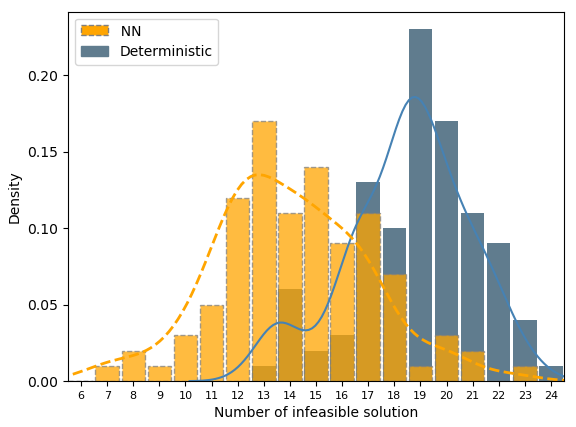
\includegraphics[width=0.9\columnwidth]{figure/fig5.png} % 
\caption{Comparing the number of infeasible solutions between NN and deterministic RP}
\label{fig5}
\end{figure}
\begin{figure}[t]
\centering
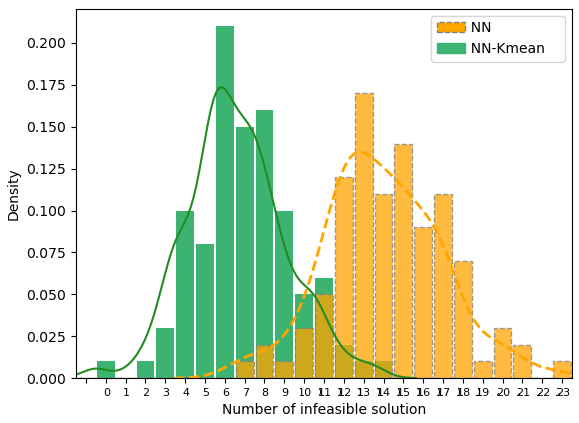
\includegraphics[width=0.9\columnwidth]{figure/fig6.png} % 
\caption{Comparing the number of infeasible solutions between NN-Kmean and NN}
\label{fig6}
\end{figure}

\begin{table}[t]
\scriptsize
\caption{The results of $t$-test for mean equality hypothesis}\smallskip
\centering
%\resizebox{.95\columnwidth}{!}{
\smallskip\begin{tabular}{ccccc}
\hline
Population  & T-value & \makecell{degree of \\freedom} & \makecell{Confidence \\ interval 95\%} & P-value  \\
\hline
\makecell{NN / deterministic}
 & \makecell{-12.024}
  & \makecell{198}
 & \makecell{[-5.25, -3.77]}
 & \makecell{0.0} \\
 \hline
\makecell{NN / NN-Kmean}
 & \makecell{-19.326}
  & \makecell{198}
 & \makecell{[-8.16, -6.64]}
 & \makecell{0.0} \\
 \hline
\end{tabular}
\label{table2}
\end{table}
The NN-Kmean is compared with worst-case and average scenario robust formulation in table 4. These results show that the worst-case can provide a significant improvement in the MRI\% but performance of this method with a 151\% optimality gap (in average) is not reasonable as shown in figure 5. Therefore, can be find the NN-Kmean with less than 15\% optimality gap is a practical and applicable robust optimization method with creating the trade-off between the feasibility and optimality. The optimality gap is the percentage of gap between I) the objective function of presented robust approaches and II) the objective function of the deterministic model considering the final realized data. In this case the objective function is minimizing the total system costs including setup, production and inventory holding costs. (The robust model with optimization measurement is explained in appendix)
\iffalse
The robust model with optimization measurement can be create by adding objective function (13) a constraints (14),(15) and (16) to the proposed robust model. Where $sc_{jo}$ is setup cost needed to run operation $o$ of job $j$ in each period.The $pc_{jo}$ and $hc_{jo}$ are respectively setup cost, production cost needed for one unit of operation $o$ of job $j$. The $zs_{jot}$, $zp_{jot}$ and $zh_{jot}$ are respectively setup cost, production cost and inventory holding cost variables regarding operation $o$ of job $j$ in period $t$. The $\omega$ is a penalty cost (fixed positive large number).
\fi
\begin{table}[t]
\scriptsize
\caption{Comparing the MRI between NN and NN-Kmean and deterministic approaches}\smallskip
\centering
\smallskip\begin{tabular}{ccccccc}
\hline
\multirow{2}{*}{samples} & \multicolumn{2}{c}{Deterministic}  & \multicolumn{2}{c}{NN}           & \multicolumn{2}{c}{NN-Kmean}    \\ \cline{2-7} 
                         & MRI\%           & RPD\%            & MRI\%           & RPD\%           & MRI\%           & RPD\%          \\ \hline
12-3-3                   & 73.7\%          & 173.0\%          & 45.0\%          & 66.7\%          & 27.0\%          & 0.0\%          \\
20-5-3                   & 69.3\%          & 136.5\%          & 47.3\%          & 61.4\%          & 29.3\%          & 0.0\%          \\
36-6-3                   & 63.0\%          & 117.2\%          & 45.0\%          & 87.5\%          & 29.0\%          & 0.0\%          \\
40-5-3                   & 71.7\%          & 172.6\%          & 48.7\%          & 84.8\%          & 26.3\%          & 0.0\%          \\
50-5-3                   & 67.0\%          & 114.1\%          & 43.7\%          & 39.4\%          & 31.3\%          & 0.0\%          \\ \hline
12-3-4                   & 64.0\%          & 123.0\%          & 46.3\%          & 61.6\%          & 28.7\%          & 0.0\%          \\
20-5-4                   & 72.3\%          & 151.9\%          & 51.3\%          & 79.1\%          & 28.7\%          & 0.0\%          \\
36-6-4                   & 70.7\%          & 128.1\%          & 45.7\%          & 47.3\%          & 31.0\%          & 0.0\%          \\
40-5-4                   & 70.3\%          & 160.4\%          & 49.3\%          & 82.7\%          & 27.0\%          & 0.0\%          \\
50-5-4                   & 75.0\%          & 167.9\%          & 46.7\%          & 66.7\%          & 28.0\%          & 0.0\%          \\ \hline
12-3-5                   & 72.7\%          & 190.8\%          & 44.0\%          & 76.0\%          & 25.0\%          & 0.0\%          \\
20-5-5                   & 74.3\%          & 158.9\%          & 47.7\%          & 66.3\%          & 28.7\%          & 0.0\%          \\
36-6-5                   & 67.0\%          & 118.2\%          & 52.0\%          & 69.6\%          & 30.7\%          & 0.0\%          \\
40-5-5                   & 74.0\%          & 146.7\%          & 49.0\%          & 63.3\%          & 30.0\%          & 0.0\%          \\
50-5-5                   & 68.3\%          & 173.0\%          & 48.0\%          & 65.5\%          & 29.0\%          & 0.0\%          \\ \hline
\textbf{Average}         & \textbf{70.2\%} & \textbf{146.3\%} & \textbf{47.3\%} & \textbf{67.8\%} & \textbf{28.6\%} & \textbf{0.0\%} \\ \hline
\end{tabular}
\end{table}
\iffalse
\begin{equation}
Min \left(\sum_{t=1}^{T} \sum_{j=1}^{J} \sum_{o=1}^{h_{j}} zs_{jot}+zp_{jot}+zh_{jot}+\omega(ps_{jot}+pl_{jot}) \right)
\end{equation}\\
\begin{equation}
(zs_{jot} \geq sc_{jo}) \vee  \lnot(x_{jot} \geq 0) \quad\quad \forall t ,\forall (j,o)
\end{equation}
\begin{equation}
(zp_{jot} \geq pc_{jo}x_{jot}) \quad\quad \forall t ,\forall (j,o)
\end{equation}
\begin{equation}
(zh_{jot} \geq hc_{jo}I_{jot}) \quad\quad \forall t ,\forall (j,o)
\end{equation}
\fi
\begin{table}[t]
\scriptsize
\caption{Comparing the performance of NN-Kmean, worst-case scenario and average scenario}\smallskip
\centering
\begin{tabular}{llll}
\hline
Samples                 & Robust approaches & MRI\%  & RPD\%   \\ \hline
\multirow{3}{*}{20-5-3} & NN-Kmean          & 29.3\% & 95.3\%  \\
                        & Worst-case        & 15.0\% & 0.0\%   \\
                        & Average-scenario  & 61.0\% & 306.7\% \\ \hline
\multirow{3}{*}{36-6-3} & NN-Kmean          & 29.0\% & 84.7\%  \\
                        & Worst-case        & 15.7\% & 0.0\%   \\
                        & Average-scenario  & 59.3\% & 277.7\% \\ \hline
\multirow{3}{*}{20-5-4} & NN-Kmean          & 28.7\% & 120.8\% \\
                        & Worst-case        & 13.0\% & 0.0\%   \\
                        & Average-scenario  & 63.4\% & 387.7\% \\ \hline
\multirow{3}{*}{36-6-4} & NN-Kmean          & 31.0\% & 97.5\%  \\
                        & Worst-case        & 15.7\% & 0.0\%   \\
                        & Average-scenario  & 65.7\% & 382.2\% \\ \hline
\multirow{3}{*}{20-5-5} & NN-Kmean          & 28.7\% & 79.4\%  \\
                        & Worst-case        & 16.0\% & 0.0\%   \\
                        & Average-scenario  & 61.4\% & 283.8\% \\ \hline
\end{tabular}
\end{table}
\begin{figure}[t]
\centering
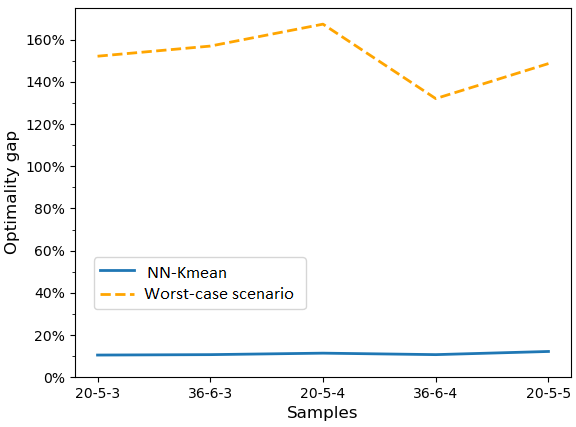
\includegraphics[width=0.9\columnwidth]{figure/fig7.png} % 
\caption{Comparing the Optimality gap between NN-Kmean and worst-case scenario approach}
\label{fig6}
\end{figure}
\section{Conclusion}
The purpose of this paper is to develop a new data-driven robust approach in lot-sizing and scheduling problems with a set of jobs that are restricted by non-permission of back-orders. Therefor, finding the feasible solution becomes more important especially considering uncertainty in unstable production environment. The robust formulation has been presented under SMT  format with regard to two resilience parameters include safety stock and safety slack. These parameters have led to the fortification of the model against the demand and processing time uncertainty. The main question is what level of safety is required for model robustness considering the current situation of the problem. To answer this question automated modeling considering different conditions of the production environment is developed using Machine learning. The combination of a regression neural network and a heuristic based on the K-mean clustering algorithm has been developed to the interpretation of uncertainty distribution function so that the nominal value and variation amplitude of random parameters have been extracted by them respectively. The computational results that are provided based on a Monte Carlo simulation show the robustness and effectiveness of the proposed approach so that in average more than 140\% improvement in number of infeasible solutions is achieved. Extending the model to formulate more assumptions of real case production plants is one straightforward opportunity for future research. This development could be more focused on evaluating and selecting features that are affecting uncertainty distribution. Also, it may be interesting to study the applicability of the proposed ML approach to other types of robust formulation such as chance constraint or robust optimization for bounded and symmetric uncertainty.
\section{Acknowledgments}
The research has been supported by the Ministry of Education, Youth and Sports within the dedicated program ERC CZ under the project POSTMAN with reference LL1902.

\section{References}
Alem, D., Curcio, E., Amorim, P.,Almada-Lobo, B. 2018. A computational study of the general lot-sizing and scheduling model under demand uncertainty via robust and stochastic approaches. \textit{Computers \& Operations Research}, 90, 125-141.\\
Baykasoğlu, A., Ozsoydan, F. B. 2018. Dynamic scheduling of parallel heat treatment furnaces: A case study at a manufacturing system. \textit{Journal of manufacturing systems}, 46, 152-162.\\
Berral, J. L., Goiri, Í., Nou, R., Julià, F., Guitart, J., Gavaldà, R., Torres, J. 2010. Towards energy-aware scheduling in data centers using machine learning. In  \textit{Proceedings of the 1st International Conference on energy-Efficient Computing and Networking}, 215-224.\\
Bitran, G. R., Yanasse, H. H. 1982. Computational complexity of the capacitated lot size problem.  \textit{Management Science}, 28(10), 1174-1186.\\
Curcio, E., Amorim, P., Zhang, Q., Almada-Lobo, B. 2018. Adaptation and approximate strategies for solving the lot-sizing and scheduling problem under multistage demand uncertainty.  \textit{International Journal of Production Economics}, 202, 81-96.\\
de León, A. D., Lalla-Ruiz, E., Melián-Batista, B., Moreno-Vega, J. M. 2017. A machine learning-based system for berth scheduling at bulk terminals.  \textit{Expert Systems with Applications}, 87, 170-182.\\
Dolgui, A., Grimaud, F., Shchamialiova, K. 2010. Supply chain management under uncertainties: lot-sizing and scheduling rules.  \textit{Artificial Intelligence Techniques for Networked Manufacturing Enterprises Management}, 181-220. Springer, London.\\
Drexl, A., Kimms, A. 1997. Lot sizing and scheduling—survey and extensions.  \textit{European Journal of operational research}, 99(2), 221-235.\\
Gupta, D., Maravelias, C. T., Wassick, J. M. 2016. From rescheduling to online scheduling.  \textit{Chemical Engineering Research and Design}, 116, 83-97.\\
Haase, K., Kimms, A. 2000. Lot sizing and scheduling with sequence-dependent setup costs and times and efficient rescheduling opportunities.  \textit{International Journal of Production Economics}, 66(2), 159-169.\\
He, S., Sim, M., Zhang, M. 2019. Data-driven patient scheduling in emergency departments: A hybrid robust-stochastic approach.  \textit{Management Science}, 65(9), 4123-4140.\\
Hu, Z., Hu, G. 2016. A two-stage stochastic programming model for lot-sizing and scheduling under uncertainty.  \textit{International Journal of Production Economics}, 180, 198-207.\\
Jiang, R., Guan, Y. 2016. Data-driven chance constrained stochastic program.  \textit{Mathematical Programming}, 158(1-2), 291-327.\\
Jin, Y., Wang, H., Chugh, T., Guo, D., Miettinen, K. 2018. Data-driven evolutionary optimization: an overview and case studies.  \textit{IEEE Transactions on Evolutionary Computation}, 23(3), 442-458.\\
Li, Y., Hu, G. 2017. Shop floor lot-sizing and scheduling with a two-stage stochastic programming model considering uncertain demand and workforce efficiency.  \textit{Computers \& Industrial Engineering}, 111, 263-271.\\
Maes, J., McClain, J. O., Van Wassenhove, L. N. 1991. Multilevel capacitated lotsizing complexity and LP-based heuristics.  \textit{European Journal of Operational Research}, 53(2), 131-148.\\
Metan, G., Sabuncuoglu, I. 2005. A Simulation Based Learning Meachanism for Scheduling Systems. In  \textit{Proceedings of the Winter Simulation Conference}, 2148-2156. IEEE.\\
Mönch, L., Zimmermann, J., Otto, P. 2006. Machine learning techniques for scheduling jobs with incompatible families and unequal ready times on parallel batch machines.  \textit{Engineering Applications of Artificial Intelligence}, 19(3), 235-245.\\
Mouelhi-Chibani, W., Pierreval, H. 2010. Training a neural network to select dispatching rules in real time.  \textit{Computers \& Industrial Engineering}, 58(2), 249-256.\\
Petrovic, S., Fayad, C., Petrovic, D. 2005. Job shop scheduling with lot-sizing and batching in an uncertain real-world environment.  \textit{2nd Multidisciplinary Conference on Scheduling: Theory and Applications}, 363-379.\\
Picard-Cantin, É., Bouchard, M., Quimper, C. G., Sweeney, J. 2016. Learning parameters for the sequence constraint from solutions. \textit{International Conference on Principles and Practice of Constraint Programming}, 405-420. Springer, Cham.\\
Rahdar, M., Wang, L., Hu, G. 2018. A tri-level optimization model for inventory control with uncertain demand and lead time.  \textit{International Journal of Production Economics}, 195, 96-105.\\
Ramezanian, R., Saidi-Mehrabad, M. 2013. Hybrid simulated annealing and MIP-based heuristics for stochastic lot-sizing and scheduling problem in capacitated multi-stage production system.  \textit{Applied Mathematical Modelling}, 37(7), 5134-5147.\\
Rohaninejad, M., Kheirkhah, A., Fattahi, P. 2015. Simultaneous lot-sizing and scheduling in flexible job shop problems.  \textit{The International Journal of Advanced Manufacturing Technology}, 78(1-4), 1-18.\\
Saif, U., Guan, Z., Wang, C., He, C., Yue, L., Mirza, J. 2019. Drum buffer rope-based heuristic for multi-level rolling horizon planning in mixed model production.  \textit{International Journal of Production Research}, 57(12), 3864-3891.\\
Schemeleva, K., Delorme, X., Dolgui, A., Grimaud, F. 2012. Multi-product sequencing and lot-sizing under uncertainties: A memetic algorithm.  \textit{Engineering Applications of Artificial Intelligence}, 25(8), 1598-1610.\\
Shiue, Y. R. 2009. Data-mining-based dynamic dispatching rule selection mechanism for shop floor control systems using a support vector machine approach.  \textit{International Journal of Production Research}, 47(13), 3669-3690.\\
Tiacci, L., Saetta, S. 2012. Demand forecasting, lot sizing and scheduling on a rolling horizon basis.  \textit{International Journal of Production Economics}, 140(2), 803-814.\\
Vargas, V., Metters, R. 2011. A master production scheduling procedure for stochastic demand and rolling planning horizons.  \textit{International Journal of Production Economics}, 132(2), 296-302.\\
Zhang, Y., Feng, Y., Rong, G. 2018a. Data-driven rolling-horizon robust optimization for petrochemical scheduling using probability density contours.  \textit{Computers \& Chemical Engineering}, 115, 342-360.\\
Zhang, Y., Jin, X., Feng, Y., Rong, G. 2018b. Data-driven robust optimization under correlated uncertainty: a case study of production scheduling in ethylene plant.  \textit{Computers \& Chemical Engineering}, 109, 48-67.\\
\end{document}
